% **************************************************
% Document Class Definition
% **************************************************
\documentclass[%
    paper=A4,               % paper size --> A4 is default in Germany
    twoside=true,           % onesite or twoside printing
    openright,              % doublepage cleaning ends up right side
    parskip=full,           % spacing value / method for paragraphs
    chapterprefix=true,     % prefix for chapter marks
    11pt,                   % font size
    headings=normal,        % size of headings
    bibliography=totoc,     % include bib in toc
    listof=totoc,           % include listof entries in toc
    titlepage=on,           % own page for each title page
    captions=tableabove,    % display table captions above the float env
    draft=false,            % value for draft version
]{scrreprt}%


% **************************************************
% Setup YOUR thesis document in this file !
% **************************************************
% !TEX root = main.tex


% **************************************************
% Files' Character Encoding
% **************************************************
\PassOptionsToPackage{utf8}{inputenc}
\usepackage{inputenc}


% **************************************************
% Information and Commands for Reuse
% **************************************************
\newcommand{\thesisTitle}{Ranking of Classification Algorithms in AutoML}
\newcommand{\thesisName}{Helena Graf}
\newcommand{\thesisSubject}{Bachelor’s Thesis}
\newcommand{\thesisDate}{January 5, 2018}
\newcommand{\thesisVersion}{My First Draft}

\newcommand{\thesisFirstReviewer}{Prof. Dr. Eyke Hüllermeier}
\newcommand{\thesisFirstReviewerUniversity}{\protect{Paderborn University}}
\newcommand{\thesisFirstReviewerDepartment}{Department of Computer Science}

\newcommand{\thesisSecondReviewer}{Prof. Dr. Axel-Cyrille Ngonga-Ngomo}
\newcommand{\thesisSecondReviewerUniversity}{\protect{Paderborn University}}
\newcommand{\thesisSecondReviewerDepartment}{Department of Computer Science}

\newcommand{\thesisFirstSupervisor}{Prof. Dr. Eyke Hüllermeier}
\newcommand{\thesisSecondSupervisor}{Prof. Dr. Axel-Cyrille Ngonga-Ngomo}

\newcommand{\thesisUniversity}{Paderborn University}
\newcommand{\thesisUniversityDepartment}{Department of Computer Science}
\newcommand{\thesisUniversityInstitute}{}
\newcommand{\thesisUniversityGroup}{Intelligent Systems Group (ISG)}
\newcommand{\thesisUniversityCity}{Paderborn}
\newcommand{\thesisUniversityStreetAddress}{Pohlweg 51}
\newcommand{\thesisUniversityPostalCode}{33098}

% **************************************************
% Debug LaTeX Information
% **************************************************
%\listfiles


% **************************************************
% Load and Configure Packages
% **************************************************
\usepackage[english]{babel} % babel system, adjust the language of the content
\PassOptionsToPackage{% setup clean thesis style
    figuresep=colon,%
    sansserif=false,%
    hangfigurecaption=false,%
    hangsection=true,%
    hangsubsection=true,%
    colorize=full,%
    colortheme=upbisg,%
    bibsys=biber,%
    bibfile=bib-refs,%
    bibstyle=alphabetic,%
    wrapfooter=false,%
}{cleanthesis}
\usepackage{cleanthesis}

\usepackage{mathtools}
\usepackage{amsmath}
\usepackage{amssymb}
\usepackage{amsthm}
\theoremstyle{definition}
\usepackage{tikz}
\usepackage{xcolor}

% Colour Definitions
\definecolor{uniblue}{RGB}{000,032,091}
\definecolor{unigrey}{RGB}{199,201,199}
\definecolor{uniaccentblue}{RGB}{000,163,224}

\hypersetup{% setup the hyperref-package options
    pdftitle={\thesisTitle},    %   - title (PDF meta)
    pdfsubject={\thesisSubject},%   - subject (PDF meta)
    pdfauthor={\thesisName},    %   - author (PDF meta)
    plainpages=false,           %   -
    colorlinks=false,           %   - colorize links?
    pdfborder={0 0 0},          %   -
    breaklinks=true,            %   - allow line break inside links
    bookmarksnumbered=true,     %
    bookmarksopen=true          %
}



% **************************************************
% Document CONTENT
% **************************************************
\begin{document}

% --------------------------
% rename document parts
% --------------------------
%\renewcaptionname{ngerman}{\figurename}{Abb.}
%\renewcaptionname{ngerman}{\tablename}{Tab.}
\renewcaptionname{english}{\figurename}{Fig.}
\renewcaptionname{english}{\tablename}{Tab.}

% --------------------------
% Front matter
% --------------------------
\pagenumbering{roman}			% roman page numbing (invisible for empty page style)
\pagestyle{empty}				% no header or footers
% !TEX root = ../main.tex
%
% ------------------------------------  --> cover title page
\begin{titlepage}
	\pdfbookmark[0]{Cover}{Cover}
	\flushright
	\hfill
	\vfill
	{\LARGE\thesisTitle \par}
	\rule[5pt]{\textwidth}{.4pt} \par
	{\Large\thesisName}
	\vfill
	\textit{\large\thesisDate} \\
	Version: \thesisVersion
\end{titlepage}


% ------------------------------------  --> main title page
\begin{titlepage}
	\pdfbookmark[0]{Titlepage}{Titlepage}
	\tgherosfont
	
	\begin{figure}
	\begin{minipage}[t]{8.5cm}		
	
\includegraphics[height=1.8cm]{gfx/upb_1E}\\
	\textsf{\small{\hspace*{1.3cm}Department of Electrical Engineering,\\
	\hspace*{1.3cm}Computer Science and Mathematics\\
%		\hspace*{1.3cm}Institute of Computer Science\\
		\hspace*{1.3cm}Warburger Straße 100 \\
		\hspace*{1.3cm}33098 Paderborn
		}}
	\end{minipage}
	\hfill
	\begin{minipage}[t]{4.7cm}
	
\includegraphics[height=1.8cm]{gfx/is-logo-klein}\\
	\textsf{%Institute of Computer Science\\
	\hspace*{0.1cm}\small{Intelligent Systems Group (ISG)}
	}
	\end{minipage}
	\end{figure}
	
	\centering
	%\textsf{\thesisUniversityDepartment} \\
	%\textsf{\thesisUniversityInstitute} \\
	%\textsf{\thesisUniversityGroup} \\

	\vfill
	{\large \thesisSubject} \\[5mm]
	{\LARGE \color{ctcolortitle}\textbf{\thesisTitle} \\[10mm]}
	{\Large \thesisName} \\[5mm]
	{Matriculation Number: 7011643}\\

	\vfill
	\begin{minipage}[t]{.27\textwidth}
		\raggedleft
		\textit{1. Reviewer}
	\end{minipage}
	\hspace*{15pt}
	\begin{minipage}[t]{.65\textwidth}
		{\Large \thesisFirstReviewer} \\
	  	{\small \thesisFirstReviewerDepartment} \\[-1mm]
		{\small \thesisFirstReviewerUniversity}
	\end{minipage} \\[5mm]
	\begin{minipage}[t]{.27\textwidth}
		\raggedleft
		\textit{2. Reviewer}
	\end{minipage}
	\hspace*{15pt}
	\begin{minipage}[t]{.65\textwidth}
		{\Large \thesisSecondReviewer} \\
	  	{\small \thesisSecondReviewerDepartment} \\[-1mm]
		{\small \thesisSecondReviewerUniversity}
	\end{minipage} \\[10mm]
	\begin{minipage}[t]{.27\textwidth}
		\raggedleft
		\textit{Supervisors}
	\end{minipage}
	\hspace*{15pt}
	\begin{minipage}[t]{.65\textwidth}
		\thesisFirstSupervisor\ and \thesisSecondSupervisor
	\end{minipage} \\[10mm]

	\thesisDate \\

\end{titlepage}


% ------------------------------------  --> lower title back for single page layout
\hfill
\vfill
{
	\small
	\textbf{\thesisName} \\
	\textit{\thesisTitle} \\
	\thesisSubject, \thesisDate \\
	Reviewers: \thesisFirstReviewer\ and \thesisSecondReviewer \\
	Supervisors: \thesisFirstSupervisor\ and \thesisSecondSupervisor \\[1.5em]
	\textbf{\thesisUniversity} \\
	\textit{\thesisUniversityGroup} \\
	% No institute
	%\thesisUniversityInstitute \\
	\thesisUniversityDepartment \\
	\thesisUniversityStreetAddress \\
	\thesisUniversityPostalCode\ and \thesisUniversityCity
}
		% INCLUDE: all titlepages
\cleardoublepage

\pagestyle{plain}				% display just page numbers
% !TEX root = ../my-thesis.tex
%
\pdfbookmark[0]{Abstract}{Abstract}
\chapter*{Abstract}
\label{sec:abstract}
\vspace*{-10mm}

Should abstract be included?

\vspace*{20mm}

{\usekomafont{chapter}Abstract (different language)}\label{sec:abstract-diff} \\

Und falls ja, dann zweisprachig?
		% INCLUDE: the abstracts (english and german)
\cleardoublepage
%
% !TEX root = ../my-thesis.tex
%
\pdfbookmark[0]{Acknowledgement}{Acknowledgement}
\chapter*{Acknowledgement}
\label{sec:acknowledgement}
\vspace*{-10mm}

Including acknowledgement expected or frowned upon for undergrad thesis?
 % INCLUDE: acknowledgement
\cleardoublepage
%
\setcounter{tocdepth}{2}		% define depth of toc
\tableofcontents				% display table of contents
\cleardoublepage

% --------------------------
% Body matter
% --------------------------
\pagenumbering{arabic}			% arabic page numbering
\setcounter{page}{1}			% set page counter
\pagestyle{maincontentstyle} 	% fancy header and footer

% Move from general to specific
\chapter{Introduction}
\label{sec:intro}

%% Context
% Need more automated analysis of data
The potential of big data is evident, and an increasing amount of information is collected and available for analysis - but this potential is not utilized. In a white paper, the International Data Corporation claims that in 2012, out of the 2.8 zettabytes (ZB) of available data only 3\% were tagged as to enable further processing, and only 0.5\% were analyzed \cite{gantz2012the}. A follow-up paper in 2017 projects that in 2025, 15\% of the estimated 163ZB of global data will be tagged, and approximately 3\% analyzed \cite{gantz2017data}. While this is more optimistic, it still shows that there is a huge gap between the amount of data that could potentially be used and the amount of data actually available. This indicates that the demand of data to be analyzed cannot be covered by data scientists alone, and the process is not accessible enough to non-experts. It thus calls for automation of the process in a way that not much expertise in the field of machine learning is needed to gain insights about the collected data.

% Of ML, tasks, classification is important & classifier performances vary across data sets, so it is not easy to just pick one
One of the most prominent machine learning tasks is classification: A class is assigned to an instance, for example clients of a bank may be either deemed creditworthy or not, based on factors like other existing credits or the job of the client. But selecting a fitting classifier for a new data set is difficult, since algorithm performances can vary substantially among data sets, and it is not feasible to simply apply a large number of them to empirically find a good match. For example, on a data set about the electricity prices in the Australian state New South Wales \cite{harris1999splice}, the predictive accuracy for the Multilayer Perceptron\footnote{With standard hyperparameters (L:0.3,M:0.2,N:500,V:0,S:0,E:20,H:a).} is 0.7887 \cite{cachada2017run3}. The predictive accuracy of the Random Forest\footnote{With standart hyperparameters (P:100,I:100,num-slots:1,K:0,M:1.0,V:0.001,S:1).} algorithm on the same data set is 0.9236 \cite{cachada2017run}, a much higher value. On a different data set, with the topic of vehicle silhouettes \cite{siebert1987vehicle}, we get a predictive accuracy of 0.7979 for the Multilayer Perceptron \cite{cachada2017run4}, and 0.7518 for Random Forests \cite{cachada2017run2}, showing an advantage of the former on this data set\footnote{Hyperparameters as above.}. So in each case, one would have picked a different algorithm in order to achieve the best results, and this example just illustrates the choice between two algorithms - in reality, the number of available algorithms is much larger. In general, this means that for a different data set, a different algorithm might yield the best performance.

\section{Problem Statement}
\label{sec:intro:problem}
%% Problem + Significance
Since there is no one best classifier for all data sets, it can be concluded that how well a classifier performs on a given data set is dependent on certain properties of the data set. Combined with the need for automated machine learning and the importance but difficulty of selecting a fitting classification algorithm, this calls for an approach that properties of data sets to automatically suggest well-performing classifiers for a new problem.

%% Response
% Therefore the goal is testing the this assumption if possible by using regression algos and preference learning
Thus, the aim of this thesis is the implementation and evaluation of two different approaches to ranking classification algorithms based on past-performances of the algorithms and according to properties of the data set. The two approaches include one regression-based approach that breaks down the problem of predicting a ranking into predicting a single performance value for each algorithm and then ranking them accordingly, and a preference based approach that is concerned with learning the rankings directly. Especially in the case of regression based ranking there is reason to believe that such a prediction is possible, as regression models have been used successfully to predict the performance of an algorithm dependent on the hyperparameter configuration \cite{DBLP:conf/aaai/EggenspergerHHL15}.

\section{Thesis Structure}
\label{sec:intro:structure}
%% Roadmap
The following paragraphs give an outline of the thesis structure by providing a brief summary of each chapter.

\textbf{Chapter \ref{sec:fundamentals} - \nameref{sec:fundamentals}} \\[0.2em]
% Begin with fundamentals to give a brief overview of the field of ML relevant to this thesis
First, some preliminaries are discussed. A brief overview of tasks from the field of machine learning which are relevant to this thesis is given, and methods used for evaluation are explained. 

\textbf{Chapter \ref{sec:approach} - \nameref{sec:approach}} \\[0.2em]
% Continue with description of the approach to the problem described in detail
The next chapter continues by describing the approach of this thesis for ranking classification algorithms. The two different proposed methods are contrasted. Following the details of the approach, the implementation thereof is presented. Used software libraries are pointed out.

% How the conducted experiments have been set up and discussion of results
\textbf{Chapter \ref{sec:evaluation} - \nameref{sec:evaluation}} \\[0.2em]
The evaluation of the different ranking implementations is described by first clarifying the experimental setup used for the evaluation, followed by a discussion of the results.

% Visit more work
\textbf{Chapter \ref{sec:related} - \nameref{sec:related}} \\[0.2em]
After the approach of this thesis has been laid out in detail, the scope is extended to related work in the area of AutoML in general and ranking of learning algorithms more specifically. Differences and similarities in the approaches are discussed briefly.

\textbf{Chapter \ref{sec:conclusion} - \nameref{sec:conclusion}} \\[0.2em]
% Conlude + future work
In the last chapter, the results which have been achieved are revisited with the goals in mind, and future work is outlined.

   % INCLUDE: introduction
\chapter{Related Work}
\label{sec:related}
% Of course much work in this field and cannot possibly cover all of this so confined to closely related or well-known / state of the art
The demand for aid in the process of selecting an algorithm has already led to the development of numerous solutions that automate machine-learning (AutoML). In the following sections, the workings of a few such tools that are related to this work are outlined briefly, loosely organized by their scope of operation. Each tool's usage of meta knowledge is discussed shortly.\\ 

\section{Predicting Rankings}
%% Ranking
% Incorporating times
In contrast to ranking solely based on classifier performances, \citeauthor{DBLP:journals/ml/AbdulrahmanBRV18} investigated an approach to extend existing ranking methods by incorporating the time needed for the evaluation of the classifier \cite{DBLP:journals/ml/AbdulrahmanBRV18}. They call this combined measure of accuracy and time A3R, and integrate it into to different ranking approaches.

% Rank aggregation A3R
One of those two approaches is called average-ranking. It utilizes meta knowledge to suggest a ranking of classifiers for a new data sets, which in this case consist of recorded past performances of classifiers on data sets. That means this algorithms aggregates the performances of classifiers on all rankings once and then always recommends the same ranking. The new measures is integrated here by, instead of ordering only according to performance values, the classifiers are ordered according to the combined measure A3R.

% Active testing A3R


% Introduce loss curves and how the measure influences them


\section{Algorithm and Hyperparameter Selection}
%% CASH
Taking it a step further than predicting rankings of classification algorithms with fixed hyperparameters are tools that in addition two selecting an algorithm also optimize its hyperparameters, which has been defined as 'the combined algorithm selection and hyperparameter optimization problem (short: CASH)' \cite{thornton2013auto}. Two widely used approaches of this kind are AUTO-WEKA and AUTO-SKLEARN. It has to be noted that thus these approaches also go further than the solution proposed in this thesis, which currently only takes into account one fixed hyperparameter configuration for each classification algorithm. 

% Auto-WEKA
Auto-WEKA is an AutoML tool that both selects a machine learning algorithm and optimizes its hyperparameters by using Bayesian optimization \cite{thornton2013auto}. It was first released in 2013 as an extension to the popular data mining software WEKA \cite{hall2009weka}, which also offers a user-friendly GUI in addition to a command-line interface and an API, to assist the large number of novice users of the software in selecting parameterized algorithms for their problems. The tool has since grown in popularity and is in version 2.0 as of March 2016 \cite{kotthoff2016auto}. In Auto-WEKA, the problem of selecting an algorithm and its hyperparameters is combined by treating the algorithm itself as a hyperparameter and searching the joint space of algorithms and hyperparameters for the best solution. An input data set is first preprocessed by means of feature selection. Then, Sequential Model-Based Optimization for General Algorithm Configuration (SMAC) is used to 'iterate[...] between fitting models and using them to make choices about which configurations to investigate' \cite{hutter2011sequential}. In the case of Auto-WEKA, this means that during the optimization process, a model is built, a configuration of hyperparameters that is promising regarding the current model and training data is tried out, and the result is fed back to the model. This cycle is then repeated until the allocated time has run out. Auto-WEKA exploits meta-knowledge, that is considering past performances of algorithms, to make decisions by always trying algorithms like Random Forest, which perform well on a large number of data sets, first. \\

% SK-learn
AUTO-SKLEARN has been described as a sister-package to Auto-WEKA and is an AutoML tool which is based on scikit-learn, a machine learning library for Python \cite{feurer2015efficient}. It works very similar to AutoML but extends it by adding a meta-learning pre-processing step to warmstart the Bayesian optimization and automatically constructing ensembles during optimization. During the pre-processing phase, performance values for the classifiers available in AUTO-SKLEARN are recorded on a set of data sets. For each data set, the algorithm which shows the best empirical performance is noted. Then, certain meta-features are calculated for each data set. The first step of the tool when given a new problem is to calculate meta-features of the data set. Then, the Manhattan distance to the other data sets is determined according to the meta-features, and the algorithms that are associated with the k-nearest data sets are used as a starting point for further optimization. The authors observe that the additional meta-learning and ensemble construction result in a more efficient and robust application. Their results show that meta-learning can be used to improve the overall AutoML process.\\

\section{Constructing pipelines}
%% Whole pipelines
Before a classifier is evaluated on a data set, often a number of pre-processing steps are executed first. These could include selecting promising features and discarding other and normalizing the data. The 'sequence of tasks that need to be performed to classify instances belonging to a given dataset into a set of predefined categories' \cite{DBLP:conf/eurogp/SaPOP17} can therefore be defined as a machine learning pipeline. Two tools which construct such complete pipelines for data sets are MP-Plan and the RECIPE framework.

% ML-Plan
ML-Plan is an AutoML tool that instead of concentrating on hyperparameter optimization, aims to optimize the whole machine-learning pipeline \cite{wever2017automatic}. This is achieved by viewing machine-learning as a task, building a hierarchical task network out of those tasks, and then searching for a solution in the induced tree structure. In the tree, the root node contains the complex task of building a machine learning pipeline, inner nodes represent incomplete pipelines consisting of complex and possibly also primitive tasks, and leaf nodes are complete pipelines that include only primitive tasks. An example of this might be 'classify' as the root node, with an intermediate node on some level that contains the tasks 'build NN', 'train NN' and 'predict from NN'. The complex task 'build NN' would then further be decomposed, and could lead to a leaf node with n tasks 'Add layer', 'build NN' and 'predict from NN', which are all primitive tasks that do not need to be further decomposed. A best-first search algorithm in a modified variant is then used to find good solutions in this task network. For the actual implementation of the learning algorithms, WEKA is used. While this variant does not use meta-learning in the process of optimizing the pipeline, the authors find that their results exceed those achieved by Auto-WEKA.\\

\tikzsetnextfilename{MLPlanTasks}
\begin{figure}
\tikzset{edge from parent/.style={draw,->}}
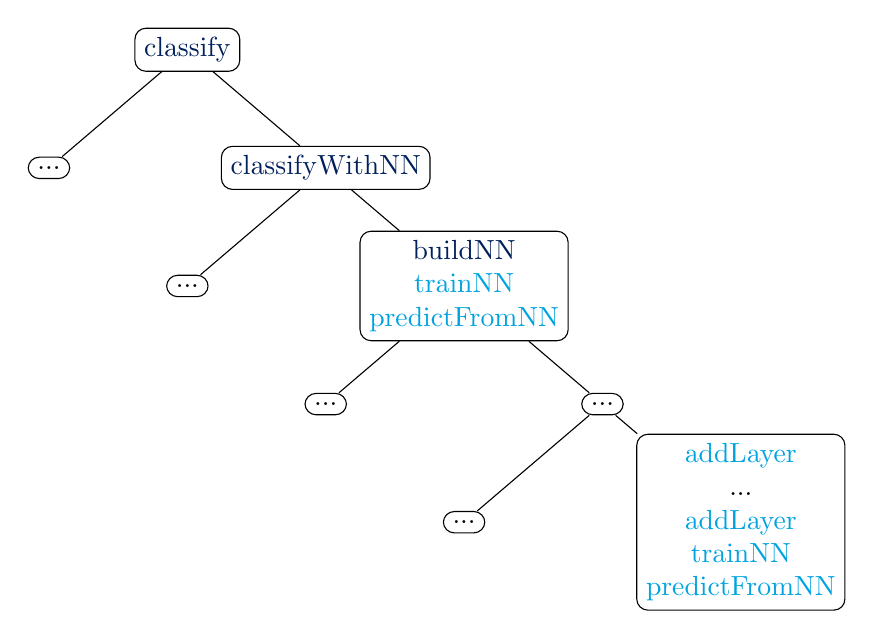
\begin{tikzpicture}[sibling distance=10em,
  every node/.style = {shape=rectangle, rounded corners,
    draw, align=center}]]
  \node {\textcolor{uniblue}{classify}}
    child { node {...} }
    child { node {\textcolor{uniblue}{classifyWithNN}}
    child { node {...} }
      child { node {\textcolor{uniblue}{buildNN} \\ \textcolor{uniaccentblue}{trainNN} \\ \textcolor{uniaccentblue}{predictFromNN}}
        child { node {...} }
        child { node {...} 
          child { node {...}  }
          child { node {\textcolor{uniaccentblue}{addLayer} \\ ... \\ \textcolor{uniaccentblue}{addLayer} \\ \textcolor{uniaccentblue}{trainNN} \\ \textcolor{uniaccentblue}{predictFromNN} } } } }
    };
\end{tikzpicture}
\caption{An example for how the complex task 'classify' might be broken down by ML-Plan. The figure is loosely adapted from \cite{wever2017automatic}. Nodes containing '...' represent an undefined number of subtrees. \textcolor{uniblue}{Complex tasks} and \textcolor{uniaccentblue}{primitive tasks} are distinguished by their color.}
\label{fig:mltree}
\end{figure}

% Recipe framework
Similar to ML-PLAN, the RECIPE framework constructs whole classification pipelines for new problems \cite{DBLP:conf/eurogp/SaPOP17}. However, this is done by means of grammar-based genetic programming: the tasks that the pipeline is composed of are represented by a grammar, which 'is used to generate the initial population, as well as to constraint the crossover and mutation operations, which always need to be valid according to the grammar' \cite{DBLP:conf/eurogp/SaPOP17}. This means that generated individuals representing complete pipelines can never be invalid. So for a new data set combined with a grammar that represents the valid pipelines, the tool first initializes the first generation according to the grammar. The fitness of individuals is then evaluated by mapping them to their respective implementations in the scikit-learn framework, and a new generation is created that takes this newly gained information into account. Evaluation by the authors indicates that the RECIPE framework is able to compete with AUTO-SKLEARN and a different evolutionary approach, although it does not incorporate meta-knowledge in the search.   % INCLUDE: related work
% !TEX root = ../my-thesis.tex
%
\chapter{System}
\label{sec:system}

\cleanchapterquote{Innovation distinguishes between a leader and a follower.}{Steve Jobs}{(CEO Apple Inc.)}

\Blindtext[2][1]

\section{System Section 1}
\label{sec:system:sec1}

\Blindtext[1][2]

\begin{figure}[htb]
	
\includegraphics[width=\textwidth]{gfx/Clean-Thesis-Figure}
	\caption{Figure example: \textit{(a)} example part one, \textit{(c)} example part two; \textit{(c)} example part three}
	\label{fig:system:example1}
\end{figure}

\Blindtext[1][2]

\section{System Section 2}
\label{sec:system:sec2}

\Blindtext[1][2]

\begin{figure}[htb]
	
\includegraphics[width=\textwidth]{gfx/Clean-Thesis-Figure}
	\caption{Another Figure example: \textit{(a)} example part one, \textit{(c)} example part two; \textit{(c)} example part three}
	\label{fig:system:example2}
\end{figure}

\Blindtext[2][2]

\section{System Section 3}
\label{sec:system:sec3}

\Blindtext[4][2]

\section{Conclusion}
\label{sec:system:conclusion}

\Blindtext[2][1]
         % INCLUDE: system
% !TEX root = ../my-thesis.tex
%
\chapter{Concepts: This text is here to test a very long title, to simulate the line break behavior, to show that an extremely long tilte also works}
\label{sec:concepts}

\cleanchapterquote{Users do not care about what is inside the box, as long as the box does what they need done.}{Jef Raskin}{about Human Computer Interfaces}

\Blindtext[2][1]

\section{Concepts Section 1}
\label{sec:concepts:sec1}

\Blindtext[2][2]

\section{Concepts Section 2}
\label{sec:concepts:sec2}

\Blindtext[3][2]

\section{Concepts Section 3}
\label{sec:concepts:sec3}

\Blindtext[4][2]

\section{Conclusion}
\label{sec:concepts:conclusion}

\Blindtext[2][1]
       % INCLUDE: concepts
% Move from specific to general
% Use existing literature for confirmation, contradiction, comparison
% "Speak to introduction"
\chapter{Conclusion}
\label{sec:conclusion}
% Introductory restatement of research problems, aims / reseach question -> remin of problem + purpose and how addressed
In this thesis, the problem of predicting a ranking of classification algorithms for a new data set on the basis of meta features of the data set and past performances of the algorithms has been considered. Being able to predict a ranking of such algorithms is desirable since this potentially speeds up and simplifies the process of algorithm selection, which is important due to a rapidly increasing amount of available data, and more importantly, data that is available but has not yet been analyzed. The problem has been addressed by implementing to different approaches, regression-based and preference-based ranking, and the evaluations of both against each other, a baseline and an oracle.

% Summary of findings and limitations: what has been covered
- Results - 

% Practical applications / limitations: assess value / relevance / implications: What does it mean for theory, what for practice
On the basis of the results, it can be concluded that a causal connection exists between certain meta features of a data set and the predictive accuracy of classification algorithms for this data set, which can be exploited to a degree by regression models and label ranking models to predict a ranking of classification algorithms. A practical application of these findings may be to incorporate the implementation or parts of it in another Auto-ML tool as a search heuristic, similar to how some Auto-ML solutions like AUTO-SKLEARN already benefits from meta learning \cite{feurer2015efficient}. However, some additional work may have to be done in extension to this thesis in order for a sensible integration.

% Recommendations for future work
\section{Future Work}
\label{sec:conclusion:future}
% Has worked reasonably well -> extend evaluation


%- more careful training by hand-selecting datasets for training (but then aains is this really the real world anymore? But then again duplicates may be contained)




- use this to try to predict other measures (e.g. time needed)
- look at the loss curve + loss-time (log) curve
- further investigate the better solution
- integrate solution into other auto ml solution if sensible regarding time contraints for that solution (and accuracy)
-e.g. use A3R
- or runtime could be predicted separately by nn based on meta data \cite{DBLP:journals/corr/abs-1709-07615}
- adding feature pre-processing

% Extension of the tool
- better fitting of learning algorithms to meta data (more manual work, but of course consider danger of overfitting!

% Extended evaluation
- compare against other tools that rank r.g. the Jan van Rijn one
- deeper analysis of meta features, e.g. add some, remove some, consider trade-off time accuracy

% Use this for predicting different algorithms
So far, the evaluation of the tool has been confined to predicting algorithms for classification. Since this has been relatively successful, it could be tested whether similar predictions can also be made for other machine learning tasks like regression or clustering. 

- hyperparameters neglected here, may include standard combinations in future work (or random ones)-> possible only if id by string
- use this for regression

an average baseline like used in speeding up algo select might be better     % INCLUDE: conclusion

% --------------------------
% Back matter
% --------------------------
\appendix\cleardoublepage
% !TEX root = ../my-thesis.tex
%
\chapter{Appendix}
\label{sec:appendix}


\section{Appendix Section 1}
\label{sec:appendix:sec1}

\begin{table}[h]
	\begin{tabularx}{\textwidth}{X | X | X}
		%\hline
		Alpha		& Beta			& Gamma			\\ \hline
		0			& 1				& 2				\\ \hline
		3			& 4				& 5				\\ %\hline
	\end{tabularx}
	\label{tab:table1}
	\caption{This is a caption text.}
\end{table}
       % INCLUDE: appendix
%
{%
\setstretch{1.1}
\renewcommand{\bibfont}{\normalfont\small}
\setlength{\biblabelsep}{0pt}
\setlength{\bibitemsep}{0.5\baselineskip plus 0.5\baselineskip}
\printbibliography[nottype=online]
\printbibliography[heading=subbibliography,title={Webpages},type=online,prefixnumbers={@}]
}
\cleardoublepage

\listoffigures
\cleardoublepage

\listoftables
\cleardoublepage

% !TEX root = ../my-thesis.tex
%
\pagestyle{empty}
\hfill
\vfill
\pdfbookmark[0]{Colophon}{Colophon}
\section*{Colophon}

This thesis was typeset with \LaTeXe.
It uses the \textit{Clean Thesis} style developed by Ricardo Langner.
The design of the \textit{Clean Thesis} style is inspired by user guide documents from Apple Inc.

Download the \textit{Clean Thesis} style at \url{http://cleanthesis.der-ric.de/}.

\cleardoublepage

% !TEX root = ../my-thesis.tex
%
%************************************************
% Declaration
%************************************************
\pdfbookmark[0]{Declaration}{Declaration}
\chapter*{Declaration}
\label{sec:declaration}
\thispagestyle{empty}

You can put your declaration here, to declare that you have completed your work solely and only with the help of the references you mentioned.

\bigskip

\noindent\textit{\thesisUniversityCity, \thesisDate}

\smallskip

\begin{flushright}
	\begin{minipage}{5cm}
		\rule{\textwidth}{1pt}
		\centering\thesisName
	\end{minipage}
\end{flushright}

%*****************************************
%*****************************************

\clearpage
\newpage
\mbox{}

% **************************************************
% End of Document CONTENT
% **************************************************
\end{document}
